


\chapter{Vision transformers for fair medical federated learning }



\begin{abstract}
In this paper, we developed a federated learning method, FedMHA, to tackle the challenges of data heterogeneity and fairness in the medical domain. The method employs the Vision Transformer architecture and Multi-Head Attention mechanism, and its performance is assessed on lung cancer CT scans with various levels of data heterogeneity, as denoted by distinct $\alpha$ values. A thorough comparison of FedMHA with other advanced federated learning models, such as FedAvg, FedAvg ResNet, FedBN, and FedProx, is conducted. The results indicate that the alignment of encoder results performs better than these models, especially in highly heterogeneous settings, and is more appropriate for large-scale federated learning situations involving a greater number of clients. Additionally, the study examines the effect of incorporating weighted averaging during model aggregation, revealing that taking into account clients' training sample size can improve the overall accuracy of the federated learning system. This research underscores the significance of addressing fairness and generalization in federated learning for medical image analysis and promotes further investigation in this field.
\end{abstract}


\newpage
\section{Introduction}

The field of medical imaging faces numerous challenges and one of the primary concerns is the privacy and security of patient data. Distributed machine learning techniques like federated learning (FL) offer a solution, enabling multiple clients, such as hospitals, to collaboratively train a shared model while keeping their data on-premise. This, in turn, ensures that sensitive patient data remains private, providing an effective and secure approach to leverage large-scale distributed datasets

However, this revolutionary approach encounters significant challenges when faced with heterogeneity in data distributions among clients. As is frequently the case in real-world medical applications, different clients, e.g., hospitals or medical centwers, may possess diverse data with varying statistical characteristics. This could result from different prevalence rates of particular diseases or distinct patterns in medical datasets among the hospitals. Such statistical heterogeneity inevitably leads to non-identical and independently distributed (non-i.i.d) data across clients. Consequently, the models resulting from these heterogeneous distributions often exhibit a decrease in diagnostic accuracy and present fairness issues, particularly disadvantaging underrepresented hospitals.

Existing federated learning methods, notably the widely-used Federated Averaging (FedAvg), have limitations in handling these heterogeneous settings effectively. Various studies have tried to tackle these challenges, such as SplitAvg \cite{zhang2022splitavg} which, while promising, risks data reconstruction attacks in a federated setting, necessitating additional security measures. Hierarchical clustering techniques \cite{yeganeh2022adaptive} \cite{gao2019hhhfl} offer an alternative but introduce substantial complexity and potential overfitting due to multi-layer optimization. Furthermore, these methods are often constrained to specific data types and have yet to prove their effectiveness across a broader range of medical imaging data \cite{gao2019hhhfl}.


% \ysc{The 1st paragraph sounds like a strong motivation to be, but how are the existing works going to resolve these challenges, what are their limitations, and more importantly what's the superiority/improvement/difference of ours to them?}
To address these challenges of data heterogeneity and fairness in the domain of medical imaging, this paper introduces an innovative federated learning approach. Specifically, this approach, utilizing a vision transformer architecture with a multi-head attention mechanism, offers a more inclusive and effective solution to federated learning. It ensures data privacy while overcoming the weaknesses of existing FL methods, in part by aligning the transformer's encoder across the clients and the server, thus improving performance, especially in highly heterogeneous settings.


Our primary objectives in this study are twofold. Firstly, we aim to address the challenge of data heterogeneity in federated learning in the context of medical imaging. Secondly, we strive to design an effective federated learning approach that preserves privacy, while avoiding the complexity associated with hierarchical methods. In light of these objectives, our main contributions to the field can be summarized as follows:
\begin{itemize}

    \item 
We propose a federated learning approach based on vision transformers and multi-head attention mechanisms. This new approach aligns the transformer's encoder across the clients and the server, managing heterogeneity in the data and ensuring fairness across different clients.

    \item 
Our approach has demonstrated notable improvements over existing methods in both accuracy and fairness. Through extensive experiments, we provide evidence of its effectiveness, especially in highly heterogeneous settings.

    \item 
We contribute a comprehensive evaluation of our proposed model against various federated learning approaches and under different heterogeneity scenarios, providing a comprehensive benchmark for future research in federated learning for medical imaging.

\end{itemize}
\section{Problem setting and background}
\textbf{Preliminaries of federated learning}
 Federated learning  has emerged as a decentralized approach for preserving data privacy and confidentiality while enabling models to learn from multiple data sources \cite{zhang2021subgraph}.
 In federated learning, each client owns a local private dataset ${D}_i$ drawn from distribution $\mathbb{P}_i(x,y)$, where $x$ and $y$ denote the input features and corresponding class labels, respectively. Usually, clients share a model $\mathcal{F}(\omega;x)$ with the same architecture and hyperparameters. This model is parameterized by learnable weights $\omega$ and input features $x$. The objective function of FedAvg~\cite{mcmahan2017communication} is:
\begin{equation} \label{eq:sl-lossw}
\arg\min_{\omega} \sum_{i=1}^{m} \frac{|D_i|}{N} \mathcal{L}_S(\mathcal{F}(\omega; x), y),
\end{equation}
\noindent where $\omega$ is the global model's parameters, $m$ denotes the number of clients, $N$ is the total number of instances over all clients, $\mathcal{F}$ is the shared model, and $\mathcal{L}_S$ is a general definition of any supervised learning task (e.g., a cross-entropy loss).

\\\textbf{ Learning with statistical heterogeneity}
In a real-world FL environment, each client may represent a mobile phone with a specific user behavior pattern or a sensor deployed in a particular location, leading to statistical and/or model heterogeneous environment. In the statistical heterogeneity setting, $\mathbb{P}_i$ varies across clients, indicating heterogeneous input/output space for $x$ and $y$. For example, $\mathbb{P}_i$ on different clients can be the data distributions over different subsets of classes. In the model heterogeneity setting, $\mathcal{F}_i$ varies across clients, indicating different model architectures and hyperparameters. For the $i$-th client, the training procedure is to minimize the loss as defined below:
\begin{equation} \label{eq:fed-sp-loss}
\small
\arg\min_{\omega_1,\omega_2,\dots,\omega_m} \sum_{i=1}^{m} \frac{|D_i|}{N} \mathcal{L}_S(\mathcal{F}_i(\omega_i; x), y).
\end{equation}


Most existing methods cannot handle the heterogeneous settings above well. In particular, the fact that $\mathcal{F}_i$ has a different model architecture would cause $\omega_i$ to have a different format and size. Thus, the global model's parameter $\omega$ cannot be optimized by averaging $\omega_i$. 

The FedAvg algorithm, proposed by McMahan et al. \cite{mcmahan2017communication}, learns a global model by averaging local models from different parties. Methods such as FedProx \cite{li2020federated}, FOLB\cite{nguyen2020fast} and FedSplit\cite{pathak2020fedsplit} improve upon FedAvg by constraining local models to remain close to the global model. Similarly, the model-contrastive (MOON) method \cite{li2021model} minimizes contrastive distances between local and global models. Despite their strengths, FL-based methods often struggle with non-iid data distribution, prompting research into personalized FL solutions, such as FedBN \cite{li2021fedbn} and FedPer\cite{arivazhagan2019federated}. 

 
\textbf{Vision Transformers}
Dosovitskiy et al.'s Vision Transformers \cite{dosovitskiy2021image} have set benchmarks in computer vision and medical image analysis~\cite{liu2021swin,hatamizadeh2022unetr,shamshad2023transformers}. Swin Transformers~\cite{liu2021swin} enhance Vision transformers by adopting hierarchical architecture with patch merging and relative position embedding. In the medical field, Vision transformers have been intergrated in the U-shaped CNN architectures~\cite{hatamizadeh2022unetr,zhou2021nnformer}. Yet, both UNETR and nnFormer, despite their respective merits, have computational and performance limitations due to the constraints of fixed token size and limited receptive field of CNN layers, respectively.

\textbf{Federated Learning in Medical Domain}
FL, with its privacy-preserving capabilities, has found utility in numerous medical tasks\cite{kaissis2021end, wu2021federated, park2021federated, guo2021multi, rieke2020future}. Notable applications of FL in medical imaging are seen in multi-institutional brain tumor segmentation\cite{fedmed1, fedmed3}, breast density classification\cite{fedmed2}, and fMRI analysis\cite{li2020multi}. Challenges presented by non-i.i.d. data in medical imaging FL, however, remain unresolved\cite{rieke2020future}.  Non-i.i.d. data impacts FedAvg algorithm's convergence speed and ultimate performance\cite{li_convergence_2020, sattler_robust_2019}. Personalization of learning rate and batch size for clients has been demonstrated to yield significant improvements\cite{wang_federated_2019}. FedOpt\cite{reddi_adaptive_2020} extends the FedAvg algorithm and introduces adjustable gradient update strategies for client and server, integrating weight decay over server-side training rounds to reduce non-i.i.d. data error\cite{li_convergence_2020}. Strategies such as global learning of base layers while retaining classification layers privately\cite{arivazhagan_federated_2019}, and individual model tailoring by each client\cite{li_fedmd_2019} have been proposed.  



\section{Global-Local Encoder Alignment}

\subsection{Image representation in Vision Transformers}\label{sec:review}
The Vision Transformer \cite{vaswani2017attention,dosovitskiy2021image} is a prominent architecture for vision tasks that primarily relies on Multi-Head Self-Attention (MHSA) to model long-range dependencies among input features. Given an input tensor $\mathbf{X} \in \mathbb{R}^{H\times W\times C}$  where $H$, $W$, and $C$ are the height, width, and the feature dimension,  
 we first reshape $\mathbf{X}$  and define the query $\mathbf{Q}$, key $\mathbf{K}$, and value $\mathbf{V}$ as follows:
\begin{equation}
\begin{aligned}
\mathbf{X} \in \mathbb{R}^{H\times W\times C} &\to \mathbf{X} \in \mathbb{R}^{(H\times W)\times C}, \\
\mathbf{Q} = \mathbf{X}\mathbf{W}^q, \qquad
\mathbf{K} &= \mathbf{X}\mathbf{W}^k, \qquad
\mathbf{V} = \mathbf{X}\mathbf{W}^v,
\end{aligned}
\end{equation}
where $\mathbf{W}^q \in \mathbb{R}^{C\times C}$, $\mathbf{W}^k \in \mathbb{R}^{C\times C}$, and $\mathbf{W}^v \in \mathbb{R}^{C\times C}$ represent the linear transformation weight matrices, which are trainable. Assuming the input and output share the same dimensions, the traditional MHSA can be expressed as:
\begin{equation}\label{equ:mhsa}
\mathbf{A} = {\rm Softmax}(\mathbf{Q}\mathbf{K}^{\rm T} / \sqrt{d}) \mathbf{V},
\end{equation}
in which $\sqrt{d}$ means an approximate normalization, and the ${\rm Softmax}$ function is applied to the rows of the matrix.
We simplify the discussion by omitting the concept of multiple heads. In \ref{equ:mhsa}, the matrix product of $\mathbf{Q}\mathbf{K}^{\rm T}$ computes the pairwise similarity between tokens. Then, each new token is derived from a combination of all tokens based on their similarity.
Following the computation of  MHSA, a residual connection is added to facilitate optimization, as shown below:
\begin{equation}\label{equ:residual}
\begin{aligned}
\mathbf{X} \in \mathbb{R}^{(H\times W)\times C} &\to \mathbf{X} \in \mathbb{R}^{H\times W\times C}, \\
\mathbf{A'} &= \mathbf{A}\mathbf{W}^p + \mathbf{X},
\end{aligned}
\end{equation}
in which $\mathbf{W}^p\in \mathbb{R}^{C\times C}$ is a trainable weight matrix for feature projection.
%
Lastly, a multilayer perceptron (MLP) is employed to enhance the representation:
\begin{equation}\label{equ:mlp}
\mathbf{Y} = {\rm MLP}(\mathbf{A'}) + \mathbf{A'},
\end{equation}
where $\mathbf{Y}$ denotes the output of a transformer block.

It is evident that the computational complexity of MHSA (\ref{equ:mhsa}) is
\begin{equation}\label{equ:complexity}
\Omega({\rm MHSA}) = 3HWC^2 + 2H^2 W^2 C.
\end{equation}
Similarly, the space complexity (memory consumption) also includes the term of $O(H^2 W^2)$. 
As commonly known, $O(H^2 W^2)$ could become very large for high-resolution inputs.This limits the applicability of transformers for vision tasks. 


\\\textbf{Alignment via regularization} 
The high computational complexity of MHSA as shown in equation (\ref{equ:complexity}) becomes a severe challenge in large-scale vision tasks. Moreover, in a federated learning scenario, we confront another pivotal issue: the statistical heterogeneity among different local models. Specifically, each local model may learn distinct features due to varying data distribution across clients. If not handled appropriately, this heterogeneity can hinder the global model's performance. The main motivation idea is to construct a surrogate function that approximates the local behavior of the objective function, yet is simpler to minimize.

Let $f(x)$ represent a function. At a given point $x = y$, we can express its quadratic approximation as:

\begin{equation}
f(y) + \nabla f(y)^T(x-y) + \frac{1}{2\mu}|x-y|^2 ,
\end{equation}

where $\nabla f(y)$ is the gradient of the function $f$ at $y$ and $\mu$ is a positive scalar, representing the step size. In the context of our federated learning setting, this translates into a quadratic upper-bound for the local loss function $F_k(w)$ around the global weights $w^t$:

\begin{align}\label{equ:reg}
F_k(w) \leq F_k(w^t) + \nabla F_k(w^t)^T(w-w^t) + \frac{1}{2\mu}||\mathbf{W}^{q,k}-\mathbf{W}^{q,G}||^2_2 ,
\end{align}

where $\nabla F_k(w^t)$ is the gradient of the local loss function at $w^t$ and $\mu$ is a positive scalar representing the step size. This regularization term is analogous to the attention score in MHSA, controlling the contribution of each feature to the final representation. The norm $||\mathbf{W}^{q,k}-\mathbf{W}^{q,G}||^2_2$ represents the Euclidean distance between the local and global model's query matrices. This regularization term aligns the local model to the global model in the query space. 

The resulting objective function becomes:

\begin{align}\label{equ:modified_obj}
\min_w
h_k(w; ~w^{t}) = F_k(w) + \frac{\mu}{2}||\mathbf{W}^{q,k}-\mathbf{W}^{q,G}||^2_2,
\end{align}

where the term $||\mathbf{W}^{q,k}-\mathbf{W}^{q,G}||^2_2$ represents the squared Euclidean norm, aligning the local query matrix $\mathbf{W}^{q,k}$ to the global one $\mathbf{W}^{q,G}$. This term constrains the update of the local models, mitigating the issue of statistical heterogeneity. Here, the regularization term is analogous to the MHSA operation, where the contribution of each query (feature) to the final output depends on the similarity between the query and key. As in MHSA, where the attention weights are computed considering all tokens, here, the regularization term takes into account the whole model parameters. However, unlike MHSA, which calculates the similarity between tokens, here we calculate the distance between the local and global model's query matrices. This regularization strategy mirrors the attention mechanism in the Vision transformers. In the next section, we extend the alignment to the more matrices of the vision transformers, resulting in more added terms.

\subsection{Multi-Head Encoder Alignment Mechanism}

% In a federated learning environment, we have multiple clients, each with their own local model. Let's denote the local model of client $i$ as $M_i$, and the global model as $M_G$. We want develop a Multi-Head Encoder Alignment (MHEA) that aligns local model encoders with the global model encoder.

First, let's define the weight matrices of the local model $M_i$ and the global model $M_G$ as $\mathbf{W}^{q}{i}$, $\mathbf{W}^{k}{i}$, $\mathbf{W}^{v}{i}$, and $\mathbf{W}^{p}{i}$ for client $i$, and $\mathbf{W}^{q}{G}$, $\mathbf{W}^{k}{G}$, $\mathbf{W}^{v}{G}$, and $\mathbf{W}^{p}{G}$ for the global model, respectively.

Now, we can reformulate the equations (1)-(4) for each client $i$ as:

\begin{equation}
\begin{aligned}
\mathbf{Q}_i = \mathbf{X}\mathbf{W}^q_i, \qquad
\mathbf{K}_i &= \mathbf{X}\mathbf{W}^k_i, \qquad
\mathbf{V}_i = \mathbf{X}\mathbf{W}^v_i
\end{aligned}
\end{equation}

Continuing from where we left off, we can now reformulate equations (2)-(4) for each client $i$ as:

\begin{equation}
\mathbf{A}_i = {\rm Softmax}(\mathbf{Q}_i\mathbf{K}_i^{\rm T} / \sqrt{d}) \mathbf{V}_i,
\end{equation}

\begin{equation}
\begin{aligned}
\mathbf{A'}_i &= \mathbf{A}_i\mathbf{W}^p_i + \mathbf{X}_i,
\end{aligned}
\end{equation}

\begin{equation}
\mathbf{Y}_i = {\rm MLP}(\mathbf{A'}_i) + \mathbf{A'}_i,
\end{equation}

where $\mathbf{Y}_i$ denotes the output of a transformer block for the local model $M_i$.

With the MHEA method, we aim to minimize the difference between each local model encoder's weights and the global model encoder's weights. To do this, we calculate the L2 difference between each local layer's weights and the corresponding global layer's weights.

Let's denote the L2 difference between the local and global layers as $L_i^k$ for client $k$ and layer $i$. For the $Q$, $K$, and $V$ weight matrices, we compute the L2 difference as follows:

\begin{equation}
\begin{aligned}
L_{i,Q}^k &= |\mathbf{W}^{q,k}_i - \mathbf{W}^{q,G}_i|^2,
L{i,K}^k &= |\mathbf{W}^{k,k}_i - \mathbf{W}^{k,G}_i|^2,
L{i,V}^k &= |\mathbf{W}^{v,k}_i - \mathbf{W}^{v,G}_i|^2,
\end{aligned}
\end{equation}

For the MLP layers, let's denote the weight matrices as $\mathbf{W}^{MLP,k}_i$ for client $k$ and $\mathbf{W}^{MLP,G}_i$ for the global model. We compute the L2 difference for the MLP layers as follows:

\begin{equation}
L_{i,MLP}^k = |\mathbf{W}^{MLP,k}_i - \mathbf{W}^{MLP,G}_i|^2
\end{equation}

Next, we incorporate these L2 differences into the local objective function for each client $k$ and layer $i$. The modified local objective function for client $k$ and layer $i$ would be:

\begin{align}
\min_w
h_k^i(w; ~w^{t}) = F_k^i(w) + \frac{\mu}{2}\left(L_{i,Q}^k + L_{i,K}^k + L_{i,V}^k + L_{i,MLP}^k\right) ,
\end{align}

This local objective function includes both the local loss function $F_k^i(w)$ and the L2 difference between the local and global layers. The MHEA term encourages the local updates to stay close to the initial global model, addressing the issue of statistical heterogeneity and safely incorporating variable amounts of local work. The federated learning process continues for multiple rounds, with the global model sending its updated parameters to the local clients and receiving their updated parameters until a specified convergence criterion is met. 
 
% \subsection{Alignment via regularization in Vision Transformers}\label{sec:alignment}


% In this way, the local model's alignment with the global model is ensured in the parameter space of the Vision Transformer, taking into account the pairwise interactions between tokens, as in the MHSA operation. This alignment, in turn, improves the federated learning performance by efficiently managing the statistical heterogeneity in client data distributions.

 
\section{Experimental Results} 

\subsection{Dataset and Pre-processing} 

Our experiment utilized a lung cancer CT scan dataset consisting of 1,119 axial slices, each of 1 mm thickness, covering a window width of 350-1200 HU. This dataset comprises images of three distinct categories: benign, malignant, and normal. The image pool was sourced from a heterogeneous patient demographic, thus ensuring diverse pathological conditions. The dataset was further divided across ten clients, each containing varying numbers of samples to simulate a realistic federated learning scenario. Pre-processing involved a series of steps to optimize the image data for the learning process. We adopted a uniform image size of 224 x 224 pixels by cropping the original images. To augment the dataset, transformations such as random rotations and horizontal flipping were applied.

\begin{figure}[htbp]
    \centering
    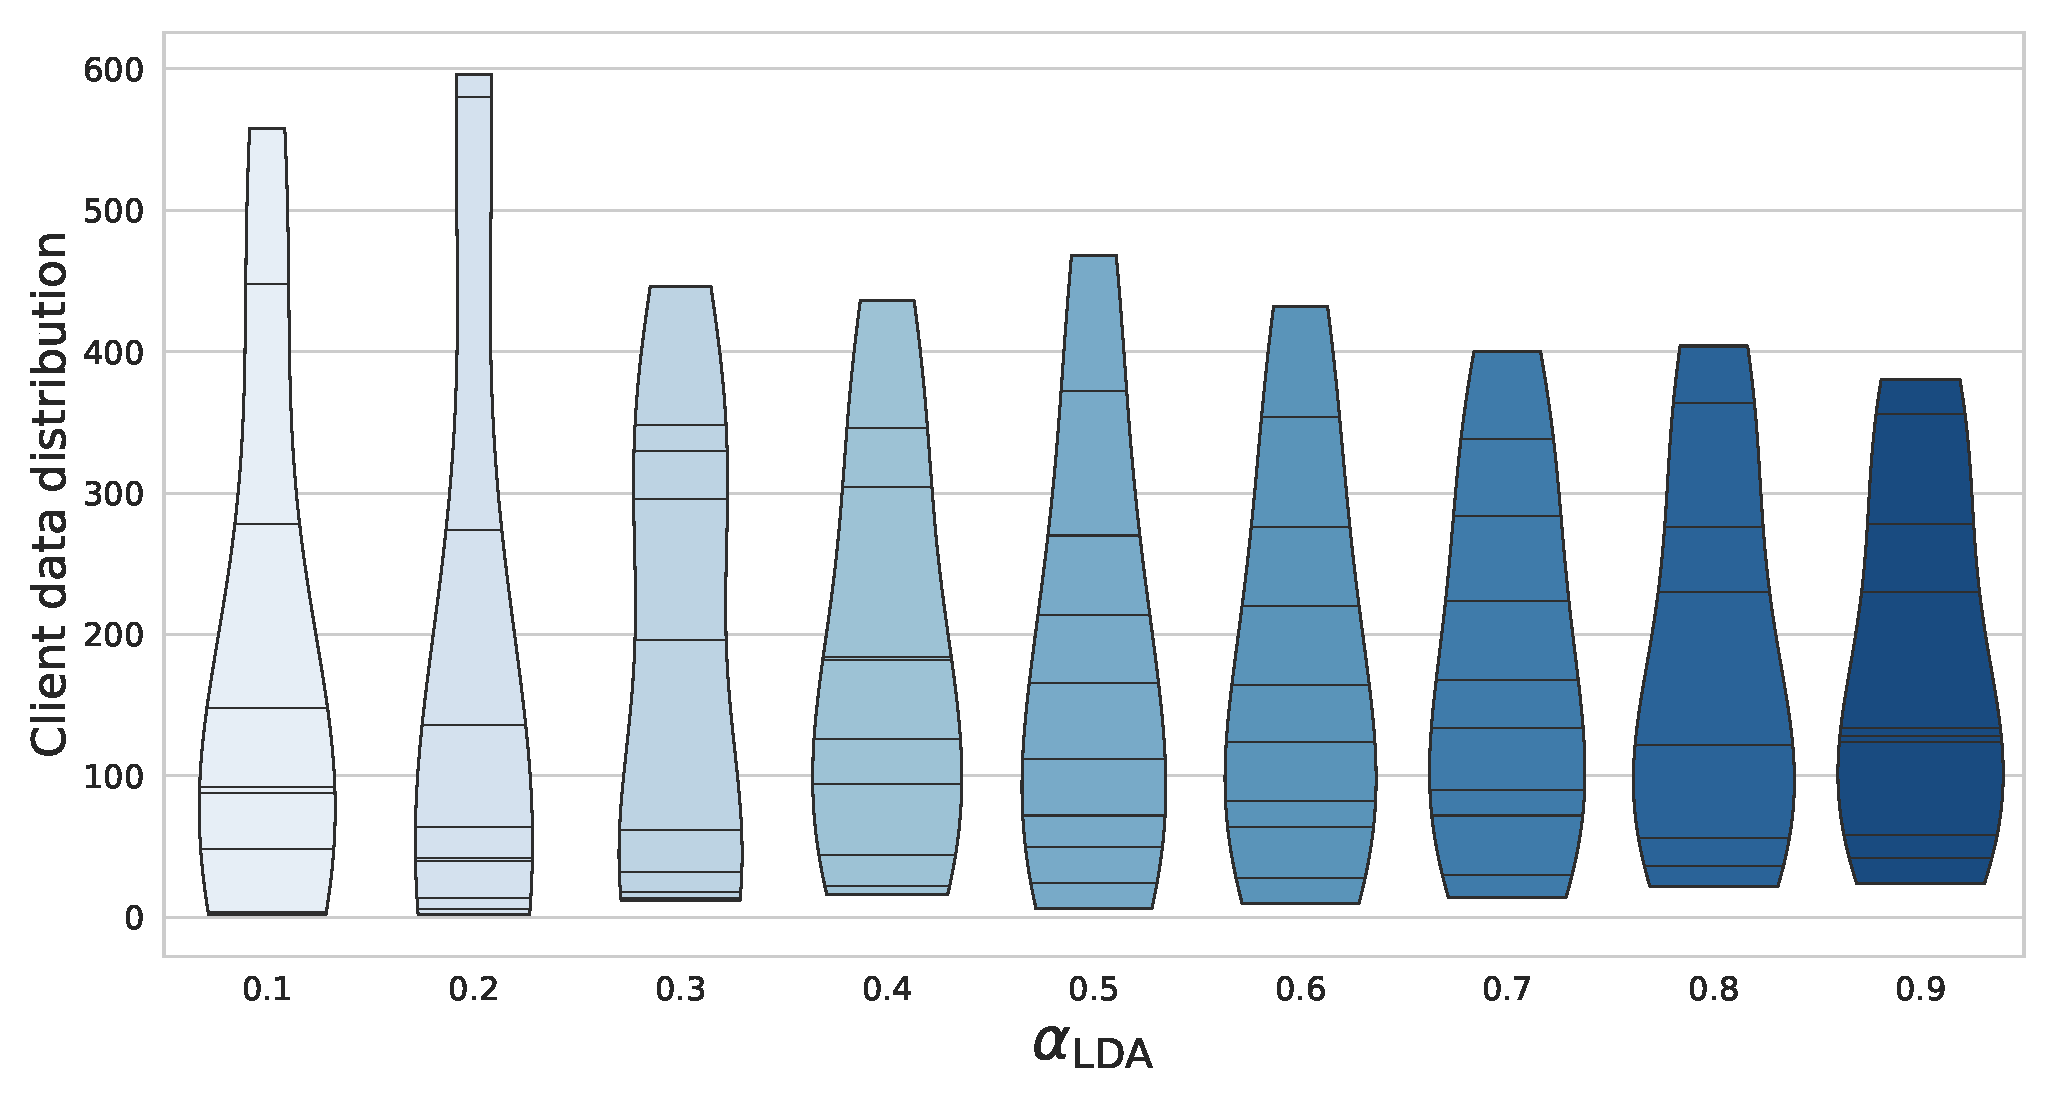
\includegraphics[width=0.7\textwidth]{violin_plot_blue_shades.eps}
   \caption{Client Data Distribution Variability at Different Heterogeneity Levels. The plot illustrates the variance in data distribution among clients as the heterogeneity levels, denoted by $\alpha$ values, alter. A longer vertical axis at lower $\alpha$ values signifies increased variability, while a wider and shorter plot at higher $\alpha$ values suggests diminished variability.}
   \label{fig:data_distribution}
\end{figure}

\subsection{Model Architectures and Training} 

Our study compared the performance of a convolutional neural network (ConvNet5) and a pre-trained vision transformer in a federated learning setting. The ConvNet5 architecture consists of five convolutional layers, each followed by batch normalization and ReLU activation function. These are succeeded by max-pooling layers and two fully connected layers with dropout to prevent overfitting.

The dataset allocation across clients was accomplished using a Latent Dirichlet Allocation (LDA) based data splitter, which is graphically represented in Figure \ref{fig:data_distribution}. Our training procedure leveraged the computational prowess of a GPU in combination with the PyTorch framework. We utilized the Stochastic Gradient Descent (SGD) optimizer with a learning rate of 0.01 and implemented gradient clipping with a max value of 5.0 to avoid exploding gradients. For FedProx method, the proximity coefficient, $\mu$, was set at 0.5. The performance of the models was evaluated using metrics such as accuracy, number of correct predictions, and loss. 

\subsection{Fairness in heterogenous settings}

\begin{figure}[htbp]
\centering
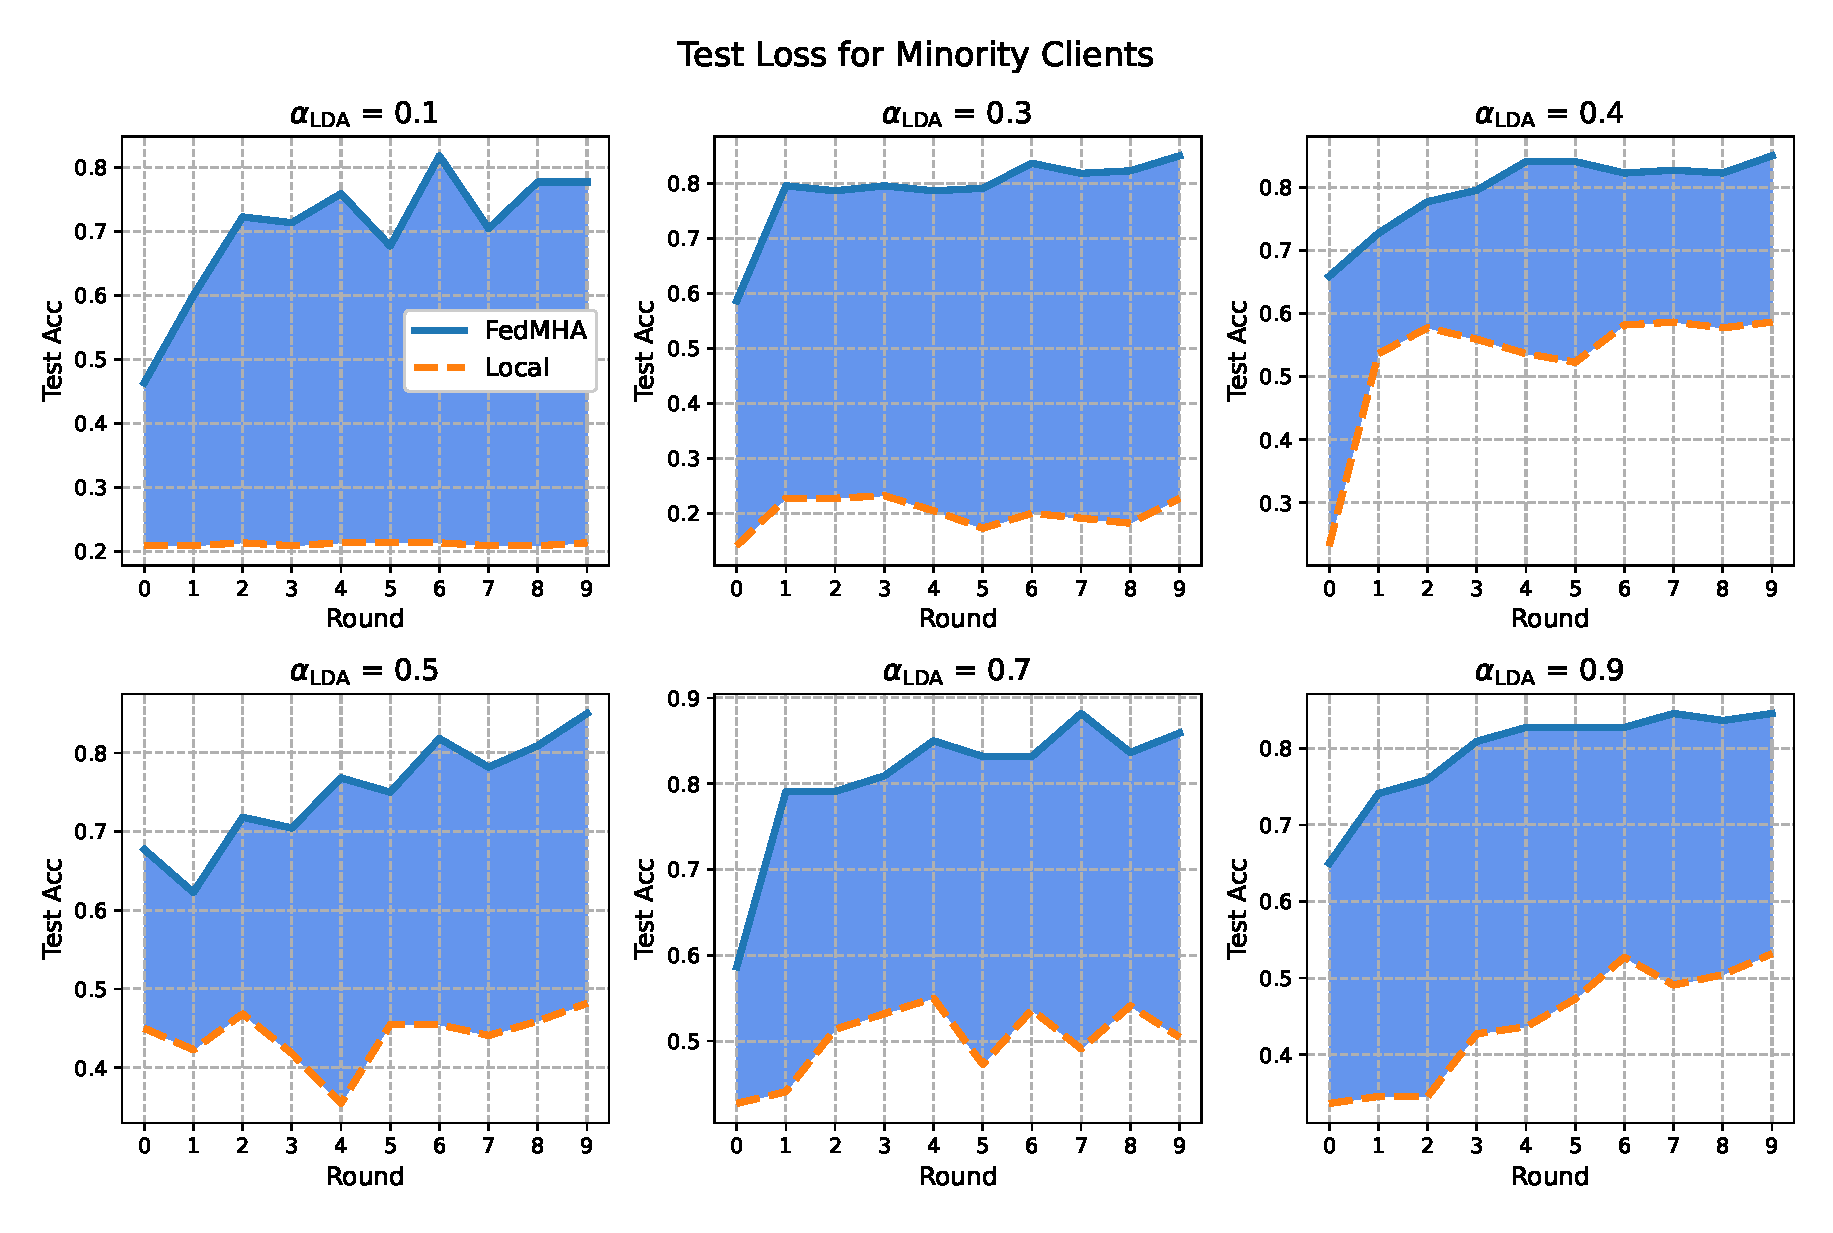
\includegraphics[width=1\textwidth,viewport=0 0 880 545,clip]{VSLocal.eps}
\caption{Performance analysis of Multi-head encoder alignment mechanism vs. Local Stochastic Gradient Descent (SGD) training across various heterogeneity levels. The graph shows higher accuracy improvement in higher heterogeneity levels.}
\label{fig:comparison_local_sgd}
\end{figure}
We evaluate the impact of our proposed model on enhancing local models for underrepresented clients as well as for all clients in terms of test accuracy improvement over different rounds. Figure \ref{fig:comparison_local_sgd} demonstrates the difference between using a Multi-head encoder alignment mechanism and local SGD training. We observed that in highly heterogeneous settings, the improvement brought about by our model was more noticeable. Furthermore, our model demonstrated faster convergence rates despite employing multiple loss functions and operating in highly heterogeneous environments. The local model typically outperformed traditional settings after the first round, indicating both higher performance and rapid convergence rates for our approach, as depicted in the provided figures.

To compare our proposed method with other federated learning algorithms , we trained the models for 10 rounds with LDA value of 0.2. Performance of each method was evaluated using a cross-entropy loss function for each round. The results were then averaged based on the number of samples per client using a weighted averaging approach. Figure \ref{fig:avg_loss_comparison} provides a comparative analysis of the average loss across various federated learning settings over the initial 10 rounds. As expected, the global model with a centralized data delivers the best performance. Following the global model, our proposed method outperforms the other federated learning algorithms, showcasing the highest average performance across multiple runs with multiple clients. FedProx and FedAvg methods exhibit lower performance, with the FedBN approach demonstrating the least satisfactory performance among the considered federated learning algorithms.


\begin{figure}[htbp]
\centering
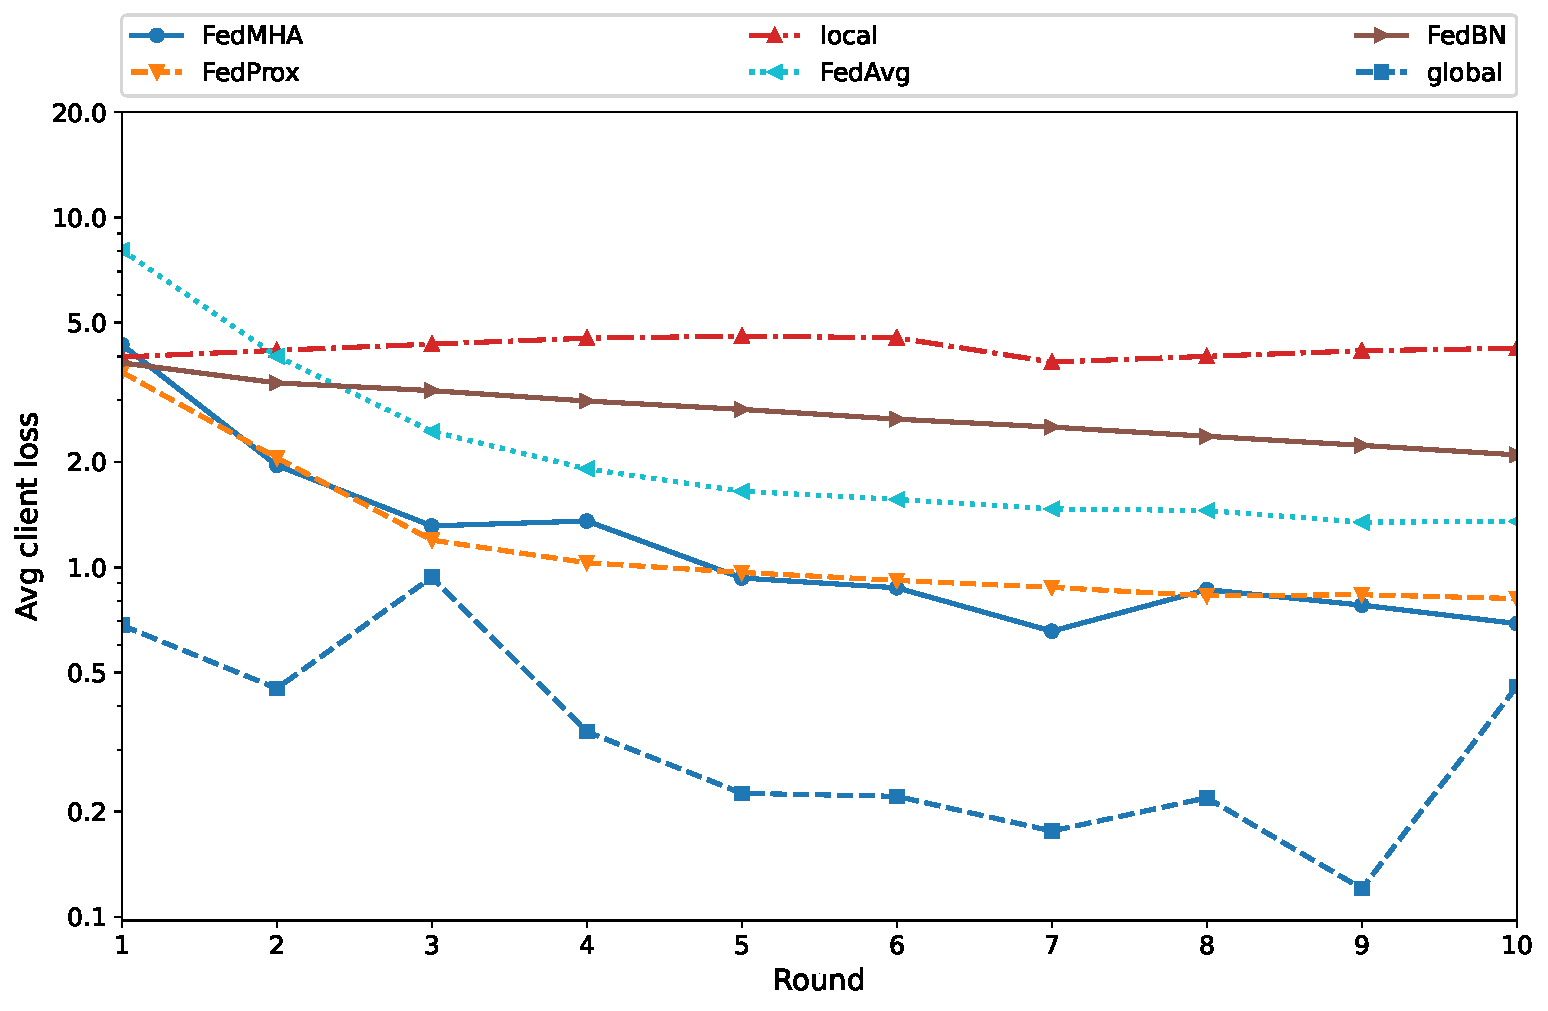
\includegraphics[width=0.7\textwidth]{plot_loss_comparison.pdf}
\caption{Comparative analysis of the average loss across various federated learning settings over the initial 10 rounds. This showcases the trajectory of client performance, with the global setting employed as a performance benchmark.}
\label{fig:avg_loss_comparison}
\end{figure} 

\subsection{Evaluation for minority clients}

In this section, we analyze the performance of minority clients in our proposed approach as shown in Figure \ref{fig:minority_performance}. The purpose of this
study is to highlight the potential struggles of minority clients in heterogeneous data environments. We trained the models independently, without exposing them to the performance of other models, and then evaluated their performance on a benchmark global dataset. Each client was trained on their own local dataset, and subsequently tested against a global dataset.

% \subsection{Effect of Varying Number of Clients}
\begin{figure}[htbp]
    \centering
    \includegraphics[width=1.13\textwidth]{test_loss_minority_clients_local.pdf}
    \caption{ Comparative loss analysis of our proposed Multi-head encoder alignment mechanism against Local SGD Training in a range of heterogeneity settings. Improved loss reduction is observed in highly heterogeneous environments when incorporating MHA, reflecting the effectiveness of our proposed method.}
    \label{fig:minority_performance}
\end{figure}



\begin{table}[h]
\centering
\caption{Comparison of federated learning methods (Local, FedMHA, FedAvg \cite{mcmahan2017communication}, FedAvg ResNet \cite{qu2022rethinking}, FedBN \cite{li2021fedbn}, FedProx \cite{li2020federated}) under different levels of data heterogeneity represented by varying $\alpha$ values. The average accuracies were calculated after 5 rounds of federated learning.}
\small % smaller font size for better fit
\setlength{\tabcolsep}{4pt} % reduce column separation
\begin{tabular}{@{}l*{7}{S[table-format=2.2,
                            table-space-text-post=\%,
                            table-column-width=12mm]}@{}}
\toprule
\rowcolor{gray!30} % color for header
\textbf{Method} & {$\alpha$ = 0.1} & {$\alpha$ = 0.2} & {$\alpha$ = 0.3} & {$\alpha$ = 0.5} & {$\alpha$ = 0.7} & {$\alpha$ = 0.8} & {$\alpha$ = 0.9} \\ 
\midrule
Local & 18.08\% & 17.85\% & 28.60\% & 46.54\% & 50.77\% & 36.67\% & 54.74\% \\ 
\addlinespace[-1pt] % reduce space above FedMHA row
\rowcolor[gray]{.9}
FedMHA & \textcolor{blue}{67.09\%} & \textcolor{blue}{74.23\%} & 70.12\% & \textcolor{blue}{81.84\%} & \textcolor{blue}{77.96\%} & \textcolor{blue}{87.76\%} & 83.99\% \\ 
\addlinespace[-1pt] % reduce space below FedMHA row
FedAvg \cite{mcmahan2017communication} & 62.03\% & 65.55\% & \textcolor{blue}{80.24\%} & 80.03\% & 72.19\% & 85.79\% & \textcolor{blue}{84.94\%} \\ 
FedAvg (ResNet50) \cite{qu2022rethinking} & 52.73\% & 61.90\% & 69.25\% & 76.88\% & 76.06\% & 85.20\% & 84.05\% \\ 
FedBN \cite{li2021fedbn} & 47.89\% & 65.97\% & 60.93\% & 63.45\% & 61.15\% & 74.05\% & 74.10\% \\ 
FedProx \cite{li2020federated} & 47.18\% & 67.42\% & 62.99\% & 72.72\% & 71.00\% & 83.89\% & 80.43\% \\ 
\bottomrule
\end{tabular}
\label{table:average_acc}
\end{table}

Table \ref{table:average_acc} provides a comparison of various federated learning methods, including our proposed FedMHA method, under different heterogeneity levels, represented by varying $\alpha$ values. The table highlights the average accuracies achieved after 5 rounds of federated learning.A detailed analysis of these results reveals that while all models generally improve their performance as the $\alpha$ value increases (corresponding to a more homogeneous data distribution), the FedMHA outperforms all other models, particularly in low $\alpha$ values. 

We conducted a side-by-side comparison with other models to analyze their performance in personalizing for various models, as shown in Figure \ref{fig:fairness_comparison}. The experiments were carried out at different alpha levels and measured the average test accuracy for all clients. Our model is represented by the blue area, while the other models are depicted with a green area. Each dot in the figure represents the mean accuracy across all clients for each level of heterogeneity. The area stretching from bottom to top illustrates the range of accuracy for the ten clients involved, with a narrower area signifying a fairer model. 
\begin{figure}[htbp]
\centering
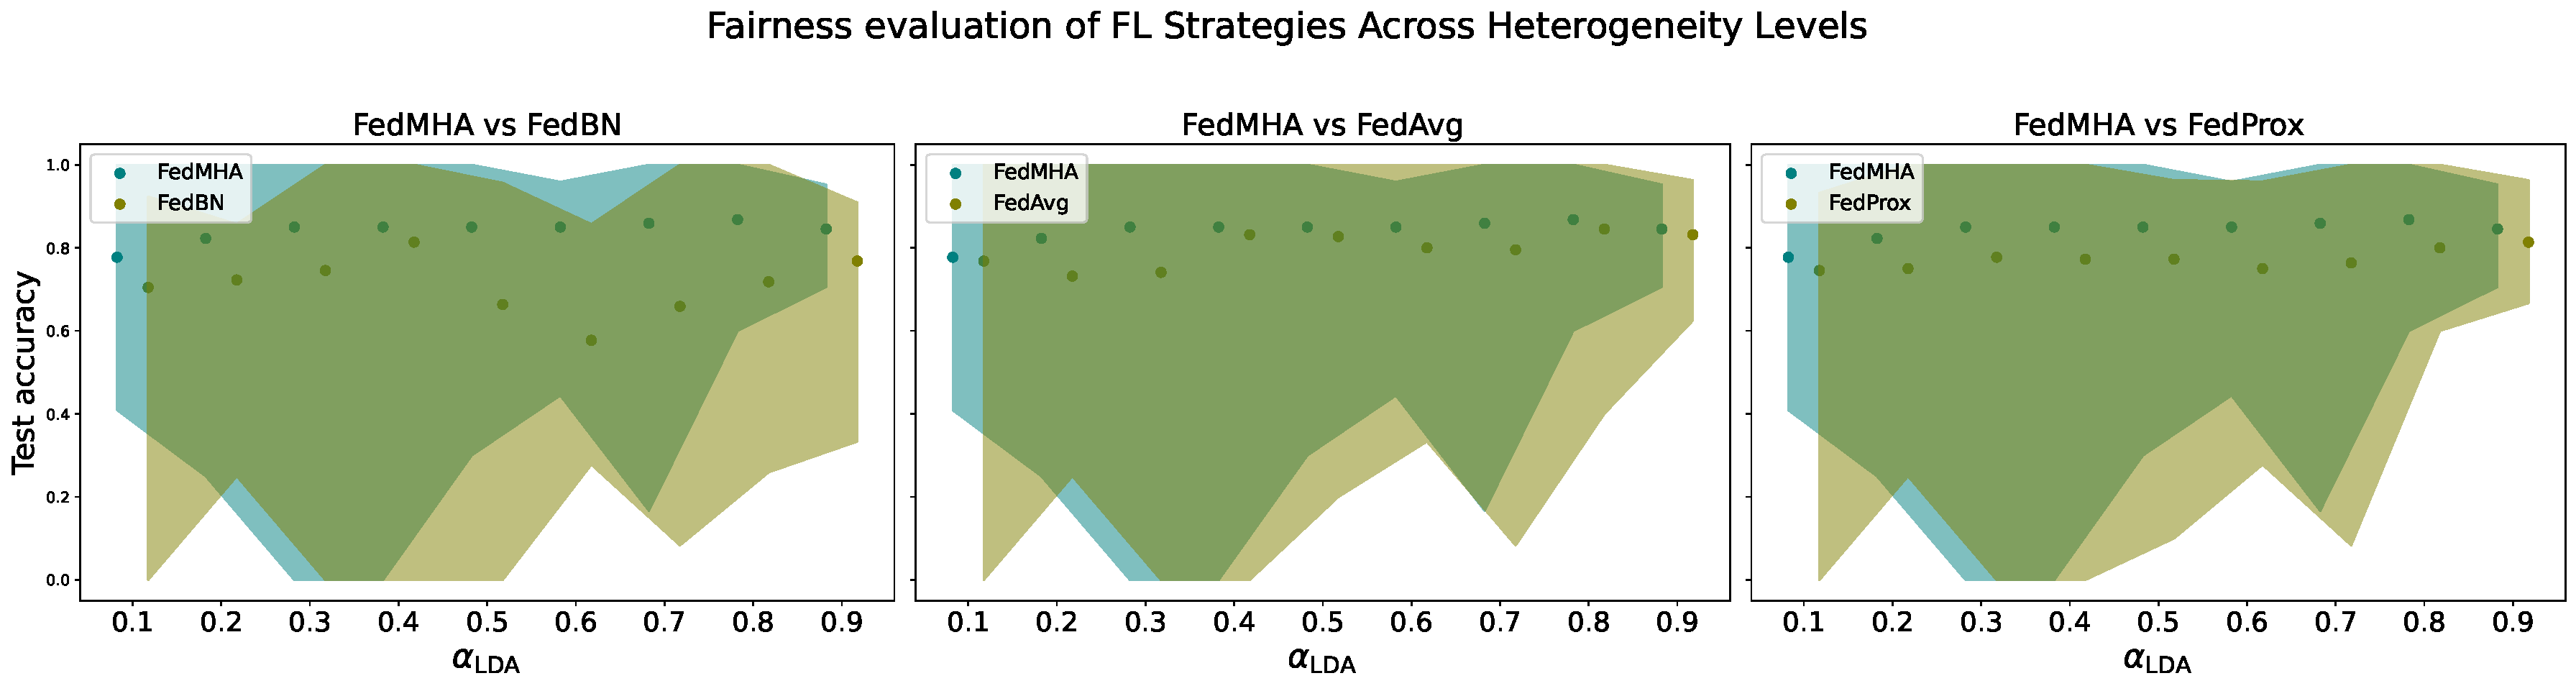
\includegraphics[width=1.15\textwidth, viewport=0 0 1800 400,clip]{comparison_plot_fairness.pdf}
\caption{Comparison of fairness in Federated Learning strategies across heterogeneity levels. Dots represent the mean accuracy for each level. The vertical stretch signifies the accuracy range for the 10 clients, with a narrower area indicating a fairer model. Our method (blue) generally outperforms other models (green), particularly in the 0.1 setting.}
\label{fig:fairness_comparison}
\end{figure}
The top line of our model is also higher, indicating that the performance of our method is  better in Vision Transformers for various clients, particularly in the 0.1 setting. The maximum accuracy achieved for these clients is around 0.4\%, while the minimum is close to zero. As the alpha value increases, the area becomes narrower, signifying that the personalization benefits are more pronounced for better-performing clients. To get a better understanding of the fairness and performance, we explore the effect of three components of our training process.

\textbf{Weighted averaging and fairness} The first component of our investigation targets the effect of the averaging paradigm. A comparison has been made between using weighted averaging, where updates from each client are weighted by the size of their respective training sample, and a more straightforward scenario where all updates are given equal weight. The results are shown in Table \ref{table:weighted_averaging}. FedMHA shows the most noticeable enhancements when weighted averaging is employed.

 \begin{table}[h]
\centering
\caption{Performance analysis of various federated learning models (FedMHA, FedAvg \cite{mcmahan2017communication}, FedAvg ResNet \cite{qu2022rethinking}, FedProx \cite{li2020federated}, FedBN \cite{li2021fedbn}, Local) with and without weighted averaging across different numbers of clients (2, 5, 8). Performance changes are compared to the FedAvg \cite{mcmahan2017communication} baseline, with improvements and declines represented by \greenuparrow{} and \reddownarrow{} respectively.}
\small % smaller font size for better fit
\setlength{\tabcolsep}{4pt} % reduce column separation
\begin{tabular}{@{}l*{6}{S[table-format=2.2,
                            table-space-text-post=\%,
                            table-column-width=14mm]}@{}}
\toprule
\rowcolor{gray!30} % color for header
\textbf{Method} & \multicolumn{3}{c}{\textbf{W/O Weighted Averaging}} & \multicolumn{3}{c}{\textbf{With Weighted Averaging}} \\
\cmidrule(lr){2-4} \cmidrule(l){5-7}
\rowcolor{gray!30} % color for sub-header
& \textbf{2 Clients} & \textbf{5 Clients} & \textbf{8 Clients} & \textbf{2 Clients} & \textbf{5 Clients} & \textbf{8 Clients} \\ 
\midrule
FedAvg \cite{mcmahan2017communication}        & 63.67\% & 61.51\% & 61.70\% & 79.55\% & 76.36\% & 76.36\% \\
FedMHA         & \ \ \textcolor{blue}{67.70\%} \greenuparrow & \ \ \textcolor{blue}{67.67\%} \greenuparrow & \ \ \textcolor{blue}{69.38\%} \greenuparrow & \ \  \textcolor{blue}{83.64\%} \greenuparrow & \  \ \textcolor{blue}{83.64\%} \greenuparrow & \ \ \textcolor{blue}{84.09\%} \greenuparrow \\
FedAvg (ResNet50) \cite{qu2022rethinking}& 60.72\% \reddownarrow & 64.96\% \greenuparrow & 64.26\% \greenuparrow & 76.36\% \reddownarrow & 80.91\% \greenuparrow & 80.00\% \greenuparrow \\
FedProx\cite{li2020federated}        & 45.73\% \reddownarrow & 59.69\% \reddownarrow & 60.58\% \reddownarrow & 58.18\% \reddownarrow & 74.55\% \reddownarrow & 75.91\% \reddownarrow \\
FedBN    \cite{li2021fedbn}   & 31.12\% \reddownarrow & 54.05\% \reddownarrow & 61.35\% \reddownarrow & 38.64\% \reddownarrow & 65.45\% \reddownarrow & 74.55\% \reddownarrow \\
\midrule
Local          & 26.20\% & 26.20\% & 26.20\% & 21.36\% & 21.36\% & 21.36\% \\
\bottomrule
\label{table:weighted_averaging}
\end{tabular}
\end{table}


\textbf{Effect of Number of Clients} As the second component, we investigate the impact of the number of clients on the performance of federated learning systems. A clear correlation emerges between the number of clients and the efficacy of federated learning models. Our proposed model, FedMHA, stands out in scenarios with a larger number of clients.  The performance improvements associated with FedMHA, both with and without weighted averaging, span an accuracy range of 67.67\% to 84.09\%. This range starkly contrasts the range of 21.36\% to 80.91\% for the other models.

\begin{figure}[htbp]
    \centering
\includegraphics[width=1.03\textwidth, viewport=0 0 1270 550,clip]{test_loss_minority_clients_fedavg.pdf}
    \caption{Impact of alignment loss on model performance. We compare the scenarios where the alignment term is retained in the local objective functions versus its removal. Models with the alignment term exhibit lower loss.}
\label{fig:Minority_loss_with_without_MHA}
\end{figure}
\textbf{Effect of alignment for underrepresented clients} The third part of our investigation looks into the influence of alignment loss on the performance of federated learning models. Here, alpha values ranging from 0.1 to 0.9 were implemented to evaluate improvements in fairness. This analysis aimed to alleviate the loss experienced by worst-performing, typically underrepresented, clients. Our approach resulted in marked enhancements, especially in settings of high heterogeneity, as shown in Figure \ref{fig:Minority_loss_with_without_MHA}. Incorporating alignment loss in the local objective functions led to a boost in local training generalization and fairness for Federated Averaging. Despite achieving satisfactory performance on training data in ideal conditions, it was observed that minority clients generally underperform in settings with high levels of data heterogeneity.
 

  


% \begin{figure}[htbp]
%     \centering
%     \includegraphics[width=1.1\textwidth]{Figures/test_loss_minority_clients_local.pdf}
%     \caption{Loss comparison}
%     \label{fig:loss_comparison}
% \end{figure}
%    \begin{figure}[htbp]
%     \centering
% \includegraphics[width=1.1\textwidth]{Figures/test_loss_minority_clients_fedavg.pdf}
%     \caption{Loss comparison}
% \label{fig:loss_comparison}
% \end{figure}




% \\
\section{Conclusion}
In this paper, we have presented and evaluated a federated learning approach that leverages Vision Transformers and multi-head attention mechanisms to effectively handle data heterogeneity in distributed settings. Our  experiments, conducted on lung cancer CT scans, demonstrate that combining optimization based approaches with vision transformer modules, outperforms existing federated learning models, particularly in scenarios with high data heterogeneity. The success of our approach in medical imaging underscores its potential in facilitating collaboration among healthcare institutions while preserving data privacy.

Our analysis  also highlights the importance of considering client data distribution and sample size during model aggregation, as a means to improve the overall accuracy. The results have implications for the medical domain, where accurate diagnosis and treatment planning are paramount. While our proposed approach exhibits superior performance in various settings, future work could focus on further enhancing fairness among clients and addressing potential scalability issues in large-scale federated learning scenarios. Additionally, exploring the use of alignment methods and vision transformers in other medical application domains could provide valuable insights into its generalizability and adaptability in the broader healthcare context.


\printbibliography